% !TEX root = /home/frank/School/thesis_text/thesis.tex



\chapter{Platform Overview}

\section{Zynq-7000}

The Zynq-7000 System on Chip combines a dual core ARM Cortex-A9 with Xilinx programmable logic in a single device. This combination of a CPU and an FPGA on the same device is not a new phenomenon, with examples of previous generations being the PowerPC based Xilinx Virtex-II Pro and some models of the Virtex 4 and Virtex 5 series FPGA's. The two most notable differences between these generations is the shift from PowerPC based architectures to ARM based architectures, and a notable shift in emphasis from HDL centered design to a more programmer centric view with an emphasis on high level languages. 
	

	\subsection{Processing System}
	The Zynq-7000 series SoC is split into two parts: The processing system (PS) and the programmable logic (PL). The Processing system (PS) contains an Application Processor Unit (APU), memory interfaces and I/O peripherals. 
	
		\paragraph{APU}
		The APU is a Dual ARM Cortex-A9 CPU which implements version 7 of the ARM ISA  as well as Thumb and Jazelle instruction sets. Each core has a NEON Media Processing Engine supporting SIMD vector and scalar single-precision floating-point and integer computation and scalar double-precision floating-point computation. Each core has 32 KB instruction and 32 KB data caches and there is 512 KB shared L2 cache and 256 KB of shard on-chip SRAM memory. The APU also has a snoop control unit to maintain L1 and L2 coherency. This snoop control unit also controls the Accelerator Coherency Port, a 64-bit AXI slave port from the programmable logic, which performs the role of master, to the processing system which serves as slave. This allows direct communication between the PS and the PL through the L2 caches or on chip memory with guaranteed coherency. The also has an on-board 8-channel DMA controller with 4-channels reserved for PS to/from memory and 4 for PL to/from memory transers. Finally the Processing system also contains an interrupt controller.

		\paragraph{Memory Controller}
		The Memory controller supports a number of memory technologies. The system has a DDR controller which supports DDR2 and DDR3 memory, a Quad-SPI controller which converts normal memory read operations to SPI and vice versa, and a Static Memory Controller which supports NAND and SRAM/NOR type memory.

		\paragraph{I/O Peripherals}
		The Processing system contains quite a lot of industry standard I/O peripherals for external data communication.
			\begin{multicols}{2}
				\begin{itemize}
					\item GPIO
					\item 2 Gigabit Ethernet Controllers
					\item 2 USB controllers
					\item 2 SD/SDIO controllers
					\item 2 SPI controllers
					\item 2 CAN controllers
					\item 2 UART controllers
					\item 2 I$^{2}$C controllers
				\end{itemize}
			\end{multicols}

		These peripherals are connected to multiplexed I/O buffers which enable to externalize these signals to up to 54 pins. If there is a need for more I/O pins the signals can be routed into the PL through the extended MIO, where they can be routed directly to package pins or peripherals in the PL.

	\subsection{Programmable Logic}
	The programmable logic provides the same functionality that can be expected from a Xilinx FPGA. The PL in 7z010 and 7z020 Zynq SoCs is based on Artix-7 FPGAs whereas the PL in 7z030, 7z045 and 7z100 SoCs is based on Kintex-7 FPGA logic. This PL can be coupled through a couple of different interconnects, with varying degrees of interconnectedness between the PL and the PS. Of note here is that the PS has to be booted first and the PL logic has to be configured from the PL at boot or at a later time. This is another example of the shift to a more software centered view. The system has all the features one can expect from an FPGA: configurable logic blocks with look-up tables, a number of 36 KB block RAMs, DSP348E slices and configurable IO. The PL side also contains an Analog to Digital converter, and in the larger varieties of the Zynq SoC an integrated PCI Express block.



\begin{figure}[H]
\centering
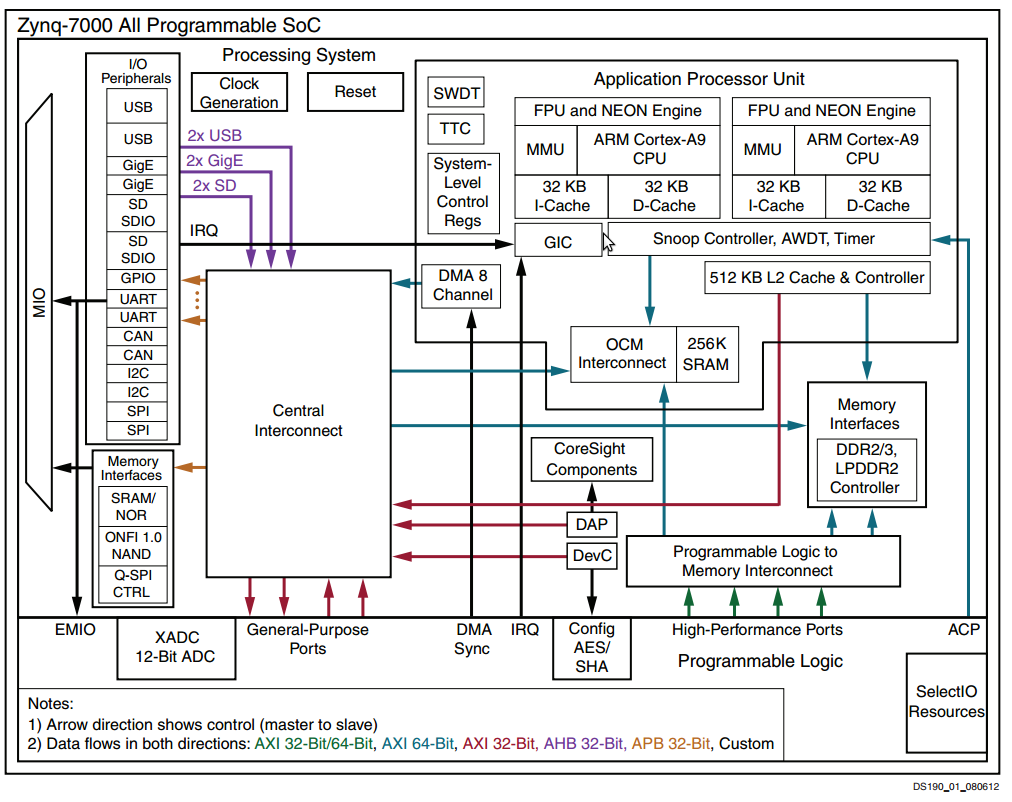
\includegraphics[scale=0.35]{/home/frank/School/thesis_text/images/zynq_overview.png}
\caption{Zynq -7000 SoC overview}
\label{img:zynq_overview}
\end{figure}

	\subsection{Interconnect}
	The interconnect system has proven to be the The Advanced Microcontroller Bus Architecture (AMBA) is an open standard specification for a bus system used in SoCs to interconnect and manage different functional blocks. 


	The AXI specification which is part of AMBA is targeted at high performance, high frequency systems. The Achilles' heel of HPC is usually costly communications. It would be interesting to research the performance of an on-chip interconnect system and a typical PCIe bus.Due to the recent launch of the zynq-7000 architecture there is little to no academic information to be found about it.\\
	Profiling for this platform is done through the Xilinx SDK software. It needs to be noted that the profiler cannot profile the hardware implemented in the programmable logic. For this other tools have to be used.[23]\\
	The board which will be used for this implementation is the Xilinx ZC702 which contains the XC7Z020 CLG484-1 AP SoC combined with the Video and Imaging kit. This contains a high definition camera and the necessary board to interface it with the SoC. 

